%
% File acl2021.tex
%
%% Based on the style files for EMNLP 2020, which were
%% Based on the style files for ACL 2020, which were
%% Based on the style files for ACL 2018, NAACL 2018/19, which were
%% Based on the style files for ACL-2015, with some improvements
%%  taken from the NAACL-2016 style
%% Based on the style files for ACL-2014, which were, in turn,
%% based on ACL-2013, ACL-2012, ACL-2011, ACL-2010, ACL-IJCNLP-2009,
%% EACL-2009, IJCNLP-2008...
%% Based on the style files for EACL 2006 by 
%%e.agirre@ehu.es or Sergi.Balari@uab.es
%% and that of ACL 08 by Joakim Nivre and Noah Smith

\documentclass[11pt,a4paper]{article}
\usepackage[hyperref]{acl2021}
\usepackage{times}
\usepackage{latexsym}
\usepackage{graphicx}

\renewcommand{\UrlFont}{\ttfamily\small}
\graphicspath{ {./images/} }

% This is not strictly necessary, and may be commented out,
% but it will improve the layout of the manuscript,
% and will typically save some space.
\usepackage{microtype}
\usepackage{booktabs}
\usepackage{float}


\aclfinalcopy % Uncomment this line for the final submission
%\def\aclpaperid{***} %  Enter the acl Paper ID here

%\setlength\titlebox{5cm}
% You can expand the titlebox if you need extra space
% to show all the authors. Please do not make the titlebox
% smaller than 5cm (the original size); we will check this
% in the camera-ready version and ask you to change it back.

\newcommand\BibTeX{B\textsc{ib}\TeX}

\title{Homework 2: Aspect-Based Sentiment Analysis}

\author{Michele Conti \\
	\texttt{conti.1599133@studenti.uniroma1.it}\\}

\date{}

\begin{document}
	\maketitle
	\section{Introduction}
	

	\section{Preprocessing}	

	\section{Models}
	\subsection{Models architecture}
	
	\subsection{Embeddings}
	
	\subsection{Embeddings aggregation}
	
	\subsection{Classification head}
	
	\section{Experiments}
	
	\subsection{Pre-trained word embeddings}
	
	\subsection{Dropout layers}
	
	\subsection{Improving the LSTM}
	
	\subsection{Bilinear layer}
	
	\subsection{POS tagging}
	
	\section{Conclusion}
	
	
	
	
	\clearpage
	\section{Figures and tables}
	All figures and tables have been intentionally placed at the end of the document, in this section, so that they don't affect the maximum limit of three pages for the text.
	
	\begin{figure}[H]
		\centering
		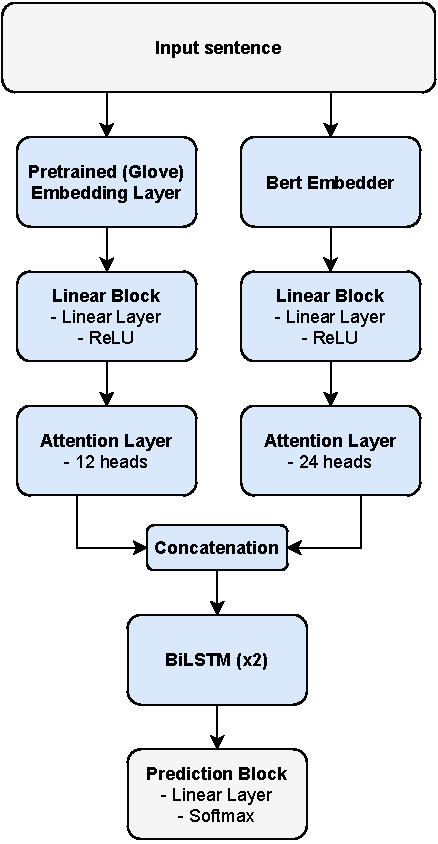
\includegraphics[width=1\columnwidth]{M3_diagram.pdf}
		\caption{M3 model architecture.}
		\label{fig:M3_architecture}
	\end{figure}
	
	\begin{table}[H]
		\centering
		\begin{tabular}{@{}lcccc@{}}
			\toprule
			\textbf{Dataset} & positive & negative & neutral & conflict \\ \midrule
			L. Train.        & 802      & 717      & 369     & 39       \\
			L. Val.          & 185      & 149      & 91      & 6        \\
			R. Train.        & 1803     & 647      & 508     & 72       \\
			R. Val.          & 361      & 158      & 125     & 19       \\ \midrule
			Train.           & 2605     & 1364     & 877     & 111      \\
			Val.             & 546      & 307      & 216     & 25       \\ \bottomrule
		\end{tabular}
		\caption{Datasets polarities frequencies (task A+B).}
		\label{tab:targets}
	\end{table}
	
	\begin{table}[H]
		\centering
		\begin{tabular}{@{}lccccc@{}}
			\toprule
			\textbf{Dataset} & anecdotes/miscellaneous & price & food & ambience & service \\ \midrule
			R. Train.        & 941                     & 268   & 1008 & 355      & 478     \\
			R. Val.          & 191                     & 53    & 224  & 76       & 119     \\ \bottomrule
		\end{tabular}
		\caption{Datasets categories frequencies (task C+D).}
		\label{tab:targets}
	\end{table}
	
	\begin{table}[H]
		\centering
		\begin{tabular}{@{}lcccc@{}}
			\toprule
			\textbf{Dataset} & positive & negative & neutral & conflict \\ \midrule
			R. Train.        & 1803     & 672      & 411     & 164      \\
			R. Val.          & 376      & 167      & 89      & 31       \\ \bottomrule
		\end{tabular}
		\caption{Datasets polarities frequencies (task C+D).}
		\label{tab:targets}
	\end{table}
	
	\bibliographystyle{acl_natbib}
	\bibliography{bibliography}
	
	%\appendix
	
	
	
\end{document}